\documentclass[a4paper,11pt,titlepage]{book}
\pdfpagewidth
\paperwidth
\pdfpageheight
\paperheight
\usepackage{subfig}
\usepackage[italian]{babel} 
\usepackage{epsfig}
\usepackage{fancyhdr} 
\usepackage{amsmath,amssymb}
\usepackage{listings}
\lstloadlanguages{python}
\usepackage{amscd} 
\usepackage[T1]{fontenc} 
\usepackage[utf8]{inputenc} 
\usepackage[usenames,dvipsnames]{xcolor}
\usepackage{graphicx,color,listings}
\usepackage{hologo}
\usepackage{amsmath}
\usepackage{amsfonts}
\usepackage[
  separate-uncertainty = true,
  multi-part-units = repeat
]{siunitx}
\frenchspacing 
\usepackage{geometry}
\usepackage{rotating}
\usepackage{caption}
\captionsetup{labelformat=empty, textfont=sl}
\geometry{a4paper,tmargin=3cm,bmargin=3cm, lmargin=3cm,rmargin=2cm} \usepackage{multirow}
\usepackage{picture}
\textwidth16cm\textheight24cm\topmargin0mm\headheight0mm\headsep6mm\oddsidemargin0mm\evensidemargin0mm


\begin{document}


\begin{center}
\textbf{{\LARGE RELAZIONE DI LABORATORIO}}
\end{center}
\vspace{1cm}
\begin{center}
Sperimentazioni di Fisica 1  Modulo B  LT Astronomia
\end{center}
\vspace{2cm}
\begin{flushleft}
\textbf{Anno accademico}: 2020/2021 \hspace{5.5cm} \textbf{Docente}: Giulia Rodighiero
\vspace{2cm}
\textbf{Gruppo di lavoro}:\\
\vspace{1cm}
Rxxxx Bxxxxxxx \hspace{0.6cm}  2xxxxxx  \hspace{0.6cm} xxxxxxxxx@studenti.unipd.it\\
\vspace{1cm}
Ixxxxx Dxxxxx \hspace{0.32cm}  2xxxxxx \hspace{0.59cm}  xxxxxxxxxxxx@studenti.unipd.it\\
\vspace{1cm}
Zambon Davide  \hspace{0.37cm} 2xxxxxx \hspace{0.6cm}  xxxxxxxxxxxxxx@studenti.unipd.it\\
\vspace{2cm}
\textbf{Data di consegna}: 30 aprile 2021
\end{flushleft}
\vspace{2cm}
\newpage







\begin{LARGE}
\begin{center}
\textbf{GUIDOVIA}
\end{center}
\end{LARGE}
\vspace*{1cm}
\begin{center}
\textbf{{\large Obiettivo dell'esperienza}} 
\end{center}
\vspace{0.15cm}
\begin{flushleft}
Lo scopo dell’esperienza consiste nell’accertare la presenza di un moto uniformemente accelerato su un piano inclinato e quindi nello stimare l’accelerazione di gravità, verificandone la compatibilità con la misura nota a Padova. 
Per piano inclinato si intende una superficie piana inclinata di un certo angolo alfa rispetto al piano orizzontale in cui, in presenza di una massa e in assenza di attrito, agiscono solamente la forza-peso e la reazione vincolare. Scomponendo queste due forze lungo le direzioni parallela e ortogonale del piano, si nota che le componenti normali si annullano, e l’unica forza attiva che rimane è la componente della forza-peso parallela al piano inclinato, di modulo costante pari a
\end{flushleft}
\begin{center}
\begin{equation}
\emph{a=gsen$\alpha$}
\end{equation}
\end{center}


\begin{flushleft}
 il moto risultante è quindi uniformemente accelerato, con accelerazione e legge oraria rispettivamente pari a
 \end{flushleft} 
 
 
\begin{center}
\begin{equation}
g=\dfrac{a}{sen{\alpha}}
\end{equation}
\end{center}

\begin{center}
\begin{equation}
s=x_0+{v_0}t+{\dfrac{1}{2}}a{t}^2
\end{equation}
\end{center}
\begin{flushleft}
L’obiettivo dell’esperienza è quindi verificare questa legge del moto.
\end{flushleft}
\vspace{0.1cm}

\includegraphics[scale=0.8]{E:/UNIPD/SPERIMEMTAZIONI FISICA 1 MOD B/relazione guidovia/immaginepianoinclinato.png} 

\newpage






\begin{center}
\begin{large}
\textbf{Descrizione dell'apparato strumentale}
\end{large}
\end{center}
\vspace{0.15cm}

\begin{flushleft}
Per la stima dell’accelerazione di gravità è stato utilizzato un piano inclinato, la guidovia, consistente in una superficie piana in alluminio a sezione rettangolare sulla quale è possibile cambiarne l’inclinazione rispetto al piano orizzontale tramite la rotazione di una vite, il cui giro completo corrisponde a 5’ (ovvero 1/12) di grado. Sulla guidovia sono stati disposti una slitta in plexiglass eventualmente equipaggiabile con un disco di ottone (in questo caso si parla di “slitta carica”) e dei traguardi a sensori infrarossi per delimitarne una regione di spazio. Per la misurazione dei tempi, invece, è stato impiegato un cronometro di precisione di sensibilità pari a 10$^{-4}$s.
\end{flushleft}
\vspace{2cm}


\begin{center}
\begin{large}
\textbf{Descrizione della metodologia della misura}
\end{large}
\end{center}
\vspace{0.15cm}


\begin{flushleft}
Dal momento che non è stato possibile recarsi in laboratorio, le misure da noi effettuate sono state prese attraverso l’utilizzo di un software chiamato “tracker” all’interno del quale sono stati caricati i video della guidovia ripresi in laboratorio dai collaboratori. Questi video riprendevano cinque spostamenti della slitta dall’inizio alla fine della guidovia per tre diverse inclinazioni: 15’, 30’ e 45’; per quest’ultima inclinazione, inoltre, è stato caricato un disco di ottone sulla slitta. Una volta caricati i video all’interno del software, sono state calibrate le lunghezze: come scala è stato utilizzato un tratto di 10cm contrassegnati grazie alla scala graduata presente sulla guidovia. Successivamente, sia sono stati collocati gli assi di riferimento cartesiani, dove l’asse delle ascisse è stato posizionato adiacente al piano orizzontale della guidovia, sia è stato contrassegnato come punto di massa il perno centrale della slitta. L’ultimo passo effettuato prima dell’effettiva presa dati è stata la taratura al tempo zero al fotogramma precedente il primo spostamento della slitta. Terminato ciò, sono stati presi posizioni e tempi della slitta lungo la guidovia ad ogni fotogramma. 
\end{flushleft}
\vspace{2cm}

\begin{flushleft}
Sono state prese ulteriori misurazioni utilizzando i video del piano inclinato creato con un asta rigida appoggiata ad un palo e facendovi scivolare un oggetto sopra. L'asta è stata inclinata di (29\SI{ \pm 1}{})° (40\SI{ \pm 1}{})°
\end{flushleft}
\newpage







\begin{center}
\begin{large}
\textbf{Presentazione dei dati sperimentali ed elaborazione dati}
\end{large}
\end{center}
\vspace{0.15cm}

\begin{flushleft}
L’elaborazione dei dati sperimentali è stata intrapresa partendo da un’analisi prettamente statistica. In primo luogo è stata calcolata la media aritmetica corrispondente ad ogni fotogramma (equivalente ad 1/3 di secondo) per ognuno dei cinque set di misurazioni relativi ad ogni inclinazione (15’, 30’, 45’ e 45’ con massa):
\end{flushleft}
\vspace{0.5cm}

\begin{equation}
\mu=\frac{1}{n}\sum\limits_{i=1}^n x_i
\end{equation}
\vspace{0.5cm}

\begin{flushleft}
dove \emph{n} rappresenta il numero di misurazioni effettuate, e \emph{xi} indica il valore di ogni singola misura.\\
\end{flushleft}

\vspace{0.5cm}
\begin{flushleft}
L’analisi statistica è proseguita con il calcolo dello scarto quadratico medio, o deviazione standard (ovvero la stima di dispersione delle misure rispetto alla media aritmetica):
\end{flushleft}

\begin{equation}
\sigma=\sqrt{\sum\limits_{i=1}^n\frac{(x_i-\mu)^2}{n-1}}
\end{equation}
\vspace{0.5cm}
\begin{flushleft}
dove $\mu$ mi indica la media aritmetica, \emph{xi} il valore di ciascuna misura e \emph{n} il numero di misurazioni effettuate.\\
\end{flushleft}
\vspace{0.5cm}

\begin{flushleft}
Successivamente è stato calcolato l'errore associato alla media:
\end{flushleft}
\vspace{0.5cm}


\begin{equation}
\sigma_\mu=\frac{\sigma }{\sqrt{n}}
\end{equation}


\vspace{0.5cm}


\begin{flushleft}
Dove $\sigma$ indica lo scarto quadratico medio e \textit{n} il valore delle misure.\\
\end{flushleft}
\vspace{0.5cm}


\begin{flushleft}
ed infine dell’errore quadratico medio:
\end{flushleft}


\begin{equation}
MSE=\dfrac{\sum\limits_{i=1}^n(x_i-\mu)^2}{n}
\end{equation}
\vspace{0.2cm}

\begin{flushleft}
dove $x_i$ è il numero di misure, $\mu$ è la media aritmetica e $n$ il numero di misure effettuate.
\end{flushleft}
\newpage


\begin{flushleft}
In secondo luogo, con l’utilizzo della funzione polyfit di Python, sono stati creati, per ogni inclinazione, dei grafici all’interno dei quali vengono rappresentati nell’asse delle ascisse i tempi e nell’asse delle ordinate gli spazi percorsi in funzione del tempo:
\end{flushleft}



\begin{figure}[h!]
\subfloat[Figura 1][parabola di bestfit con inclinazione a 15']{\includegraphics[scale=0.5]{E:/UNIPD/SPERIMEMTAZIONI FISICA 1 MOD B/relazione guidovia/figure parabole/Figure_15.png} } 
\hspace{0.2cm}
\subfloat[Figura 2][parabola di bestfit con inclinazione a 30']{\includegraphics[scale=0.5]{E:/UNIPD/SPERIMEMTAZIONI FISICA 1 MOD B/relazione guidovia/figure parabole/Figure_30.png} }\\
\subfloat[Figura 3][parabola di bestfit con inclinazione a 45']{\includegraphics[scale=0.5]{E:/UNIPD/SPERIMEMTAZIONI FISICA 1 MOD B/relazione guidovia/figure parabole/Figure_45.png} }
\hspace{0.2cm}
\subfloat[Figura 4][parabola di bestfit con inclinazione a 45' con massa sulla slitta]{\includegraphics[scale=0.5]{E:/UNIPD/SPERIMEMTAZIONI FISICA 1 MOD B/relazione guidovia/figure parabole/Figure_45M.png} }
\end{figure}
\vspace{0.5cm}

\begin{flushleft}
Osservando questi grafici, si nota che, in tutti e quattro i casi, i dati presi si dispongono su una parabola: ciò è dovuto al fatto che in un moto rettilineo uniformemente accelerato la relazione tra spostamento e tempo è quadratica, poichè siamo in presenza di un’accelerazione. La sua legge oraria è quindi (3).
\end{flushleft}
\newpage


\begin{flushleft}
Dal momento che la legge oraria esprime la differenza di spostamento in funzione del tempo, il passo successivo è stato quello di derivare le parabole ottenute, in modo da trovare la differenza di velocità al variare del tempo, ovvero la velocità istantanea, definita come:
\end{flushleft}

\begin{equation}
v(t)=at+v_0
\end{equation}
\vspace{0.2cm}

\begin{flushleft}
con $a$ accelerazione e $v$ velocità al tempo zero.
\end{flushleft}







\begin{figure}[h!]
\subfloat[Figura 1][derivata della parabola: velocità istantanea inclinazione 15']{\includegraphics[scale=0.5]{E:/UNIPD/SPERIMEMTAZIONI FISICA 1 MOD B/relazione guidovia/figure vi/vi_15.png} }
\hspace{0.2cm}
\subfloat[Figura 2][derivata della parabola: velocità istantanea inclinazione 30']{\includegraphics[scale=0.5]{E:/UNIPD/SPERIMEMTAZIONI FISICA 1 MOD B/relazione guidovia/figure vi/vi_30.png} } \\
\subfloat[Figura 3][derivata della parabola: velocità istantanea inclinazione 45']{\includegraphics[scale=0.5]{E:/UNIPD/SPERIMEMTAZIONI FISICA 1 MOD B/relazione guidovia/figure vi/vi_45.png} }
\hspace{0.2cm}
\subfloat[Figura 4][derivata della parabola: velocità istantanea inclinazione 45' con massa]{\includegraphics[scale=0.5]{E:/UNIPD/SPERIMEMTAZIONI FISICA 1 MOD B/relazione guidovia/figure vi/vi_45M.png} }
\end{figure}
\newpage











\begin{flushleft}
Osservando i grafici che riportano i valori della velocità istantanea è evidente la presenza di una relazione lineare tra la velocità e il tempo. Conoscendo la relazione fisica che sussiste tra la velocità istantanea e quella media, ovvero:
\end{flushleft}



\begin{equation}\begin{split}
\bar{v}(x_1,x_2)=&\hspace{0.2cm}\dfrac{1}{t_2-t_1}\int_{t_1}^{t_2} v(t)\, dt\\
=&\hspace{0.2cm}\dfrac{1}{t_2-t_1}\int_{t_1}^{t_2} (v_0+at)\, dt\\
=&\hspace{0.2cm}\dfrac{v_0(t_2-t_1)+\dfrac{1}{2}a({t_2}^2-{t_1}^2)}{t_2-t_1}\\
=&\hspace{0.2cm}v_0+a{\dfrac{t_1+t_2}{2}}\\
=&\hspace{0.2cm}v()\dfrac{t_1+t_2}{2}\\
=&\hspace{0.2cm}v(\bar{t})
\end{split}\end{equation}
\hspace{1cm}



\begin{flushleft}
Il passo successivo è stato l’effettivo calcolo della velocità media: 
\end{flushleft}
\vspace{1cm}

\begin{equation}
\bar{v}(x_1,x_2)=\dfrac{x_2-x_1}{t(40,x_2)-t(40,x_1)}=\dfrac{x_2-x_1}{t_2-t_1}=\dfrac{\Delta{x}}{\Delta{t}}
\end{equation}
\vspace{1cm}

\begin{flushleft}
dove $t(x_1,x_2)$ è il tempo impiegato dalla slitta per percorrere il tratto tra le coordinate $(x_1,x_2)$ e $\bar{t}$ è il tempo intermedio tra quelli in cui essa
attraversa i due punti.
\end{flushleft}
\vspace{0.2cm}



\newpage
 
 
\begin{flushleft}
Le misure delle velocità medie e delle velocità istantanee sono tutte in $m/s$.
\end{flushleft}

\begin{figure}[h!]
\subfloat[Figura 1][confronto velocità media e istantanea inclinazione 15']{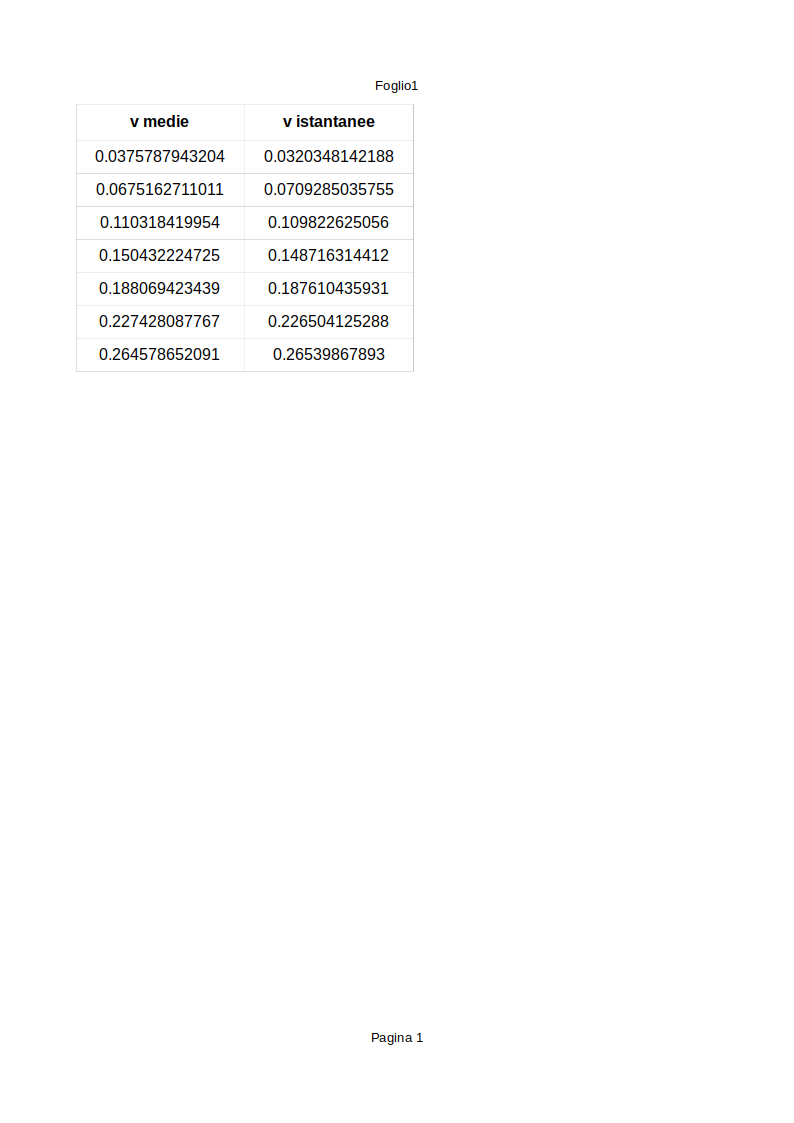
\includegraphics[scale=0.8]{E:/UNIPD/SPERIMEMTAZIONI FISICA 1 MOD B/relazione guidovia/tabelle cv/15.png} }
\vspace{0.5cm}
\hspace{0.3cm}
\subfloat[Figura 2][confronto velocità medie inclinazione e istantanea 30']{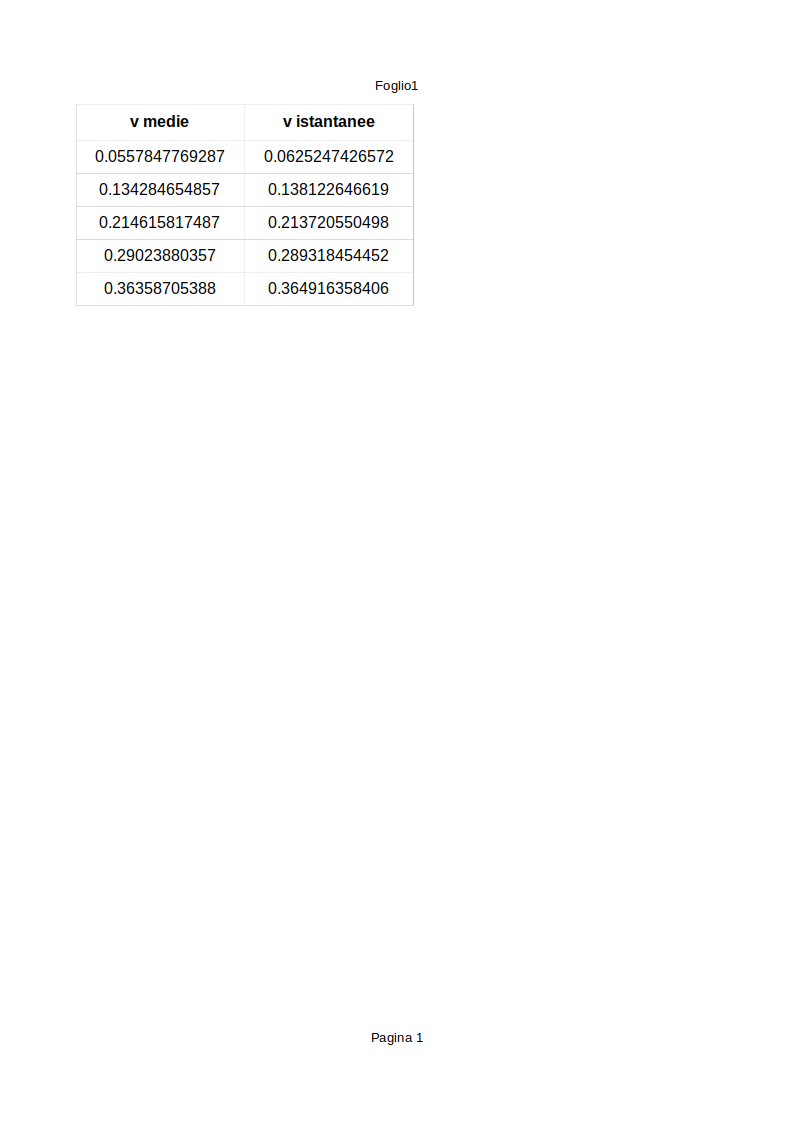
\includegraphics[scale=0.8]{E:/UNIPD/SPERIMEMTAZIONI FISICA 1 MOD B/relazione guidovia/tabelle cv/30.png} } \\
\subfloat[Figura 3][confronto velocità medie e istantanea inclinazione 45']{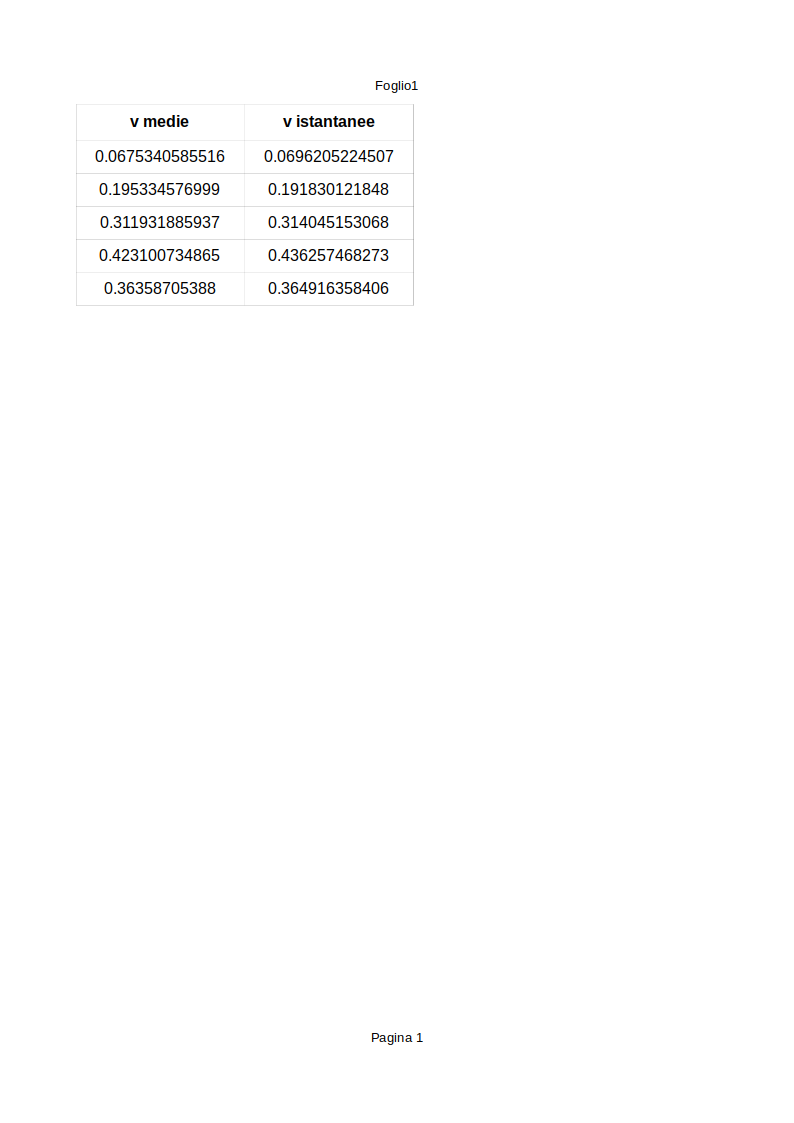
\includegraphics[scale=0.8]{E:/UNIPD/SPERIMEMTAZIONI FISICA 1 MOD B/relazione guidovia/tabelle cv/45.png} }
\vspace{0.5cm}
\hspace{0.3cm}
\subfloat[Figura 4][confronto velocità medie e istantanea inclinazione 45' con massa]{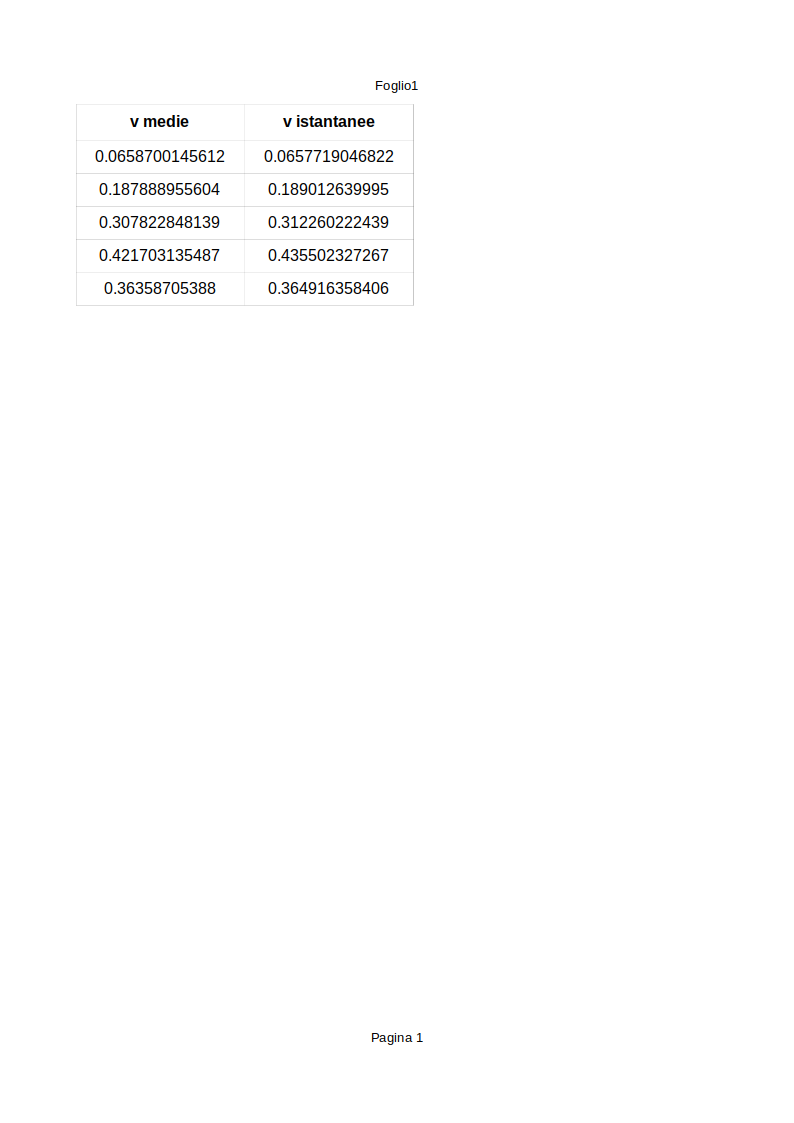
\includegraphics[scale=0.8]{E:/UNIPD/SPERIMEMTAZIONI FISICA 1 MOD B/relazione guidovia/tabelle cv/45massa.png} }
\end{figure}







\begin{flushleft}
Sapendo tuttavia che quest’ultima deve coincidere con la velocità istantanea della slitta nell’istante centrale tra i due estremi, ogni video è stato suddiviso in blocchi di 10 secondi, ovvero in intervalli di 30 fotogrammi ed è stata calcolata la velocità media nel punto intermedio di questo intervallo temporale, corrispondente a 15 fotogrammi. Effettuati i calcoli, le velocità medie e quelle istantanee relative ad ogni inclinazione, sono state disposte nello stesso grafico in modo da confermare effettivamente la loro uguaglianza.
\end{flushleft}

\vspace{2cm}





\begin{figure}[h!]
\subfloat[Figura 1][confronto velocità media e velocità istantanea inclinazione 15' di grado]{\includegraphics[scale=0.5]{E:/UNIPD/SPERIMEMTAZIONI FISICA 1 MOD B/relazione guidovia/figure cv/cv15.png} }
\hspace{0.3cm}
\subfloat[Figura 2][confronto velocità media e velocità istantanea inclinazione 30' di grado]{\includegraphics[scale=0.5]{E:/UNIPD/SPERIMEMTAZIONI FISICA 1 MOD B/relazione guidovia/figure cv/cv30.png} }\\
\subfloat[Figura 3][confronto velocità media e velocità istantanea inclinazione 45' di grado]{\includegraphics[scale=0.5]{E:/UNIPD/SPERIMEMTAZIONI FISICA 1 MOD B/relazione guidovia/figure cv/cv45.png} }
\hspace{0.3cm}
\subfloat[Figura 4][confronto velocità media e velocità istantanea inclinazione 45' con massa]{\includegraphics[scale=0.5]{E:/UNIPD/SPERIMEMTAZIONI FISICA 1 MOD B/relazione guidovia/figure cv/cv45M.png} }
\end{figure}
\newpage


\begin{flushleft}
Dai grafici si nota che le rette che rappresentano le velocità medie in funzione del tempo sono sovrapponibili a quelle delle velocità istantanee precedentemente calcolate. Quindi l’andamento delle velocità è descritto da una funzione di tipo lineare:
\end{flushleft}

\begin{equation}
y=a+bx
\end{equation}
\newpage

\begin{flushleft}
Definita questa relazione, sono stati calcolati i coefficienti $A$ e $B$ delle rette interpolanti ed i relativi errori $\sigma{a}$ e $\sigma{b}$ mediante il metodo dei minimi quadrati, nonchè l’errore sulla retta stessa $\sigma{y}$:
\end{flushleft}
\vspace{1cm}



\begin{equation}
\Delta=N{{\sum{{x}^2}}-{\sum{x}}^2}\\
\end{equation}
\vspace{0.2cm}
\begin{equation}
A=\dfrac{{\sum{{x}^2}}{\sum{y}}-{\sum{x}}{\sum{xy}}}{\Delta}\\
\end{equation}
\vspace{0.2cm}
\begin{equation}
B=\dfrac{N{\sum{xy}}-{\sum{x}}{\sum{y}}}{\Delta}\\
\end{equation}
\vspace{0.2cm}
\begin{equation}
\sigma_y=\sqrt{{\dfrac{1}{N-2}}{\sum\limits_{i=1}^n{({y_i}-{A}-{Bx_i})^2}}}\\
\end{equation}
\vspace{0.2cm}
\begin{equation}
\sigma_A=\sigma_y{\sqrt{\dfrac{\sum{{x}^2}}{\Delta}}}
\end{equation}
\vspace{0.2cm}
\begin{equation}
\sigma_B=\sigma_y\sqrt{\dfrac{N}{\Delta}}
\end{equation}

\vspace{1cm}









\begin{flushleft}
Il coefficiente b delle rette interpolanti, esprime il valore dell’accelerazione della slitta lungo la guidovia. Ricordando che in un piano inclinato l’accelerazione è data da $a=gsen\alpha$, è ora possibile stimare per tutte le inclinazioni i valori dell’accelerazione di gravità g ed i relativi errori $\sigma{g}$ utilizzando la formula $g=a/sen\alpha$ e la propagazione degli errori rispettivamente.
\end{flushleft}




\newpage
\begin{flushleft}
I valori così ottenuti sono: 
\end{flushleft}
\vspace{1cm}



\begin{figure}[h!]
\subfloat[Figura 1][valori di $g$ guidovia]{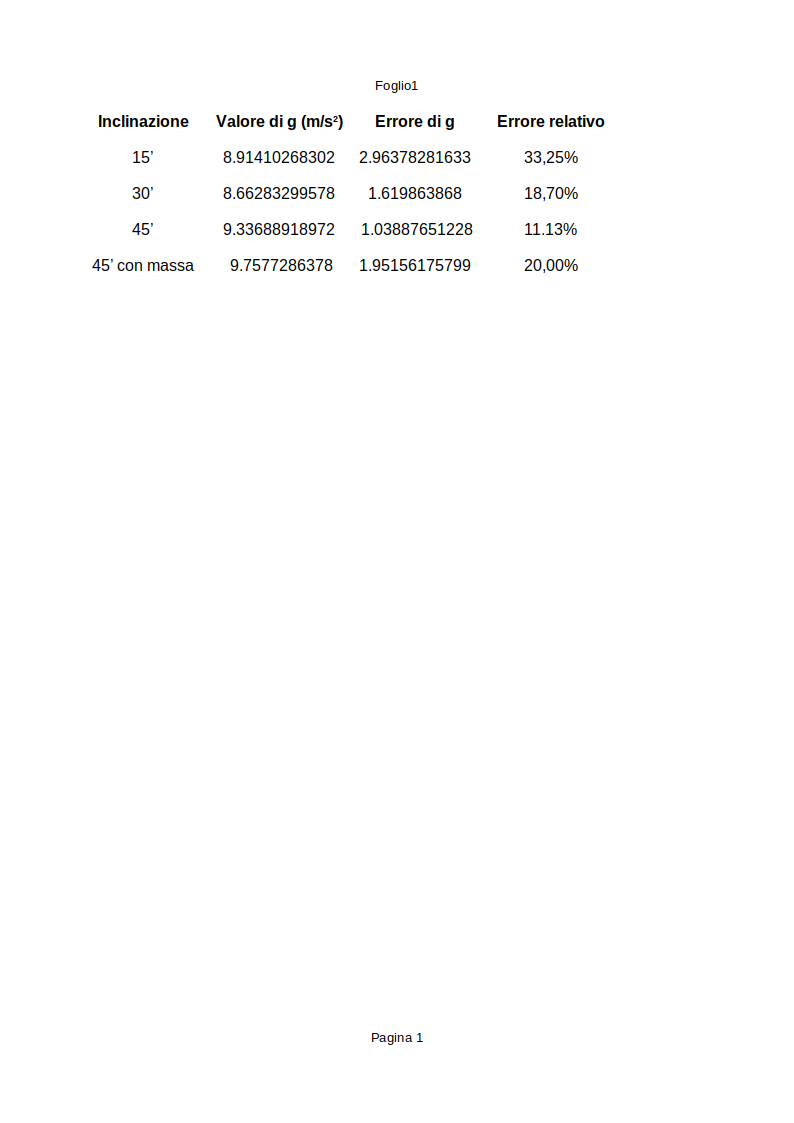
\includegraphics[scale=0.8]{valori di g.png} }
\end{figure}

\vspace{1cm}

\begin{figure}[h!]
\subfloat[Figura b][valori di $g$ sistema asta-palo]{\includegraphics[scale=0.8]{valori di g brutto.png} }
\end{figure}























\newpage
\begin{center}
\begin{large}
\textbf{Discussione dei dati sperimentali}
\end{large}
\end{center}

\vspace{0.15cm}

\begin{flushleft}
Confrontando i risultati delle quattro stime dell’accelerazione di gravità calcolate per ogni inclinazione, si osserva che i valori ottenuti non si discostano eccessivamente rispetto al valore atteso a Padova, pari a mettere valore gravità; tuttavia, gli errori relativi riferiti alle quattro misurazioni superano il 10$\%$. Questa discrepanza, è dovuta al fatto che le misurazioni effettuate sono accurate, ma non precise. La scarsa precisione è data dalla notevole presenza di errori casuali dovuti alla difficoltà nel raccoglimento dei dati con il software “tracker”, soprattutto nel primo tratto della guidovia dove, la distanza tra uno spostamento e quello successivo ad ogni fotogramma risultava essere molto piccola.
\end{flushleft}



\vspace{1cm}
\begin{flushleft}
Con lo stesso procedimento utilizzato per la guidovia abbiamo calcolato $g$ a partire dai dati del sistema asta-palo. I risultati ottenuti risentono della forza di attrito, per questo motivo il valore di $g$ è notevolmente smorzato rispetto a quello stimato a Padova, in misura tanto maggiore quanto più il piano si avvicina all'orizzontale.
\end{flushleft}



\begin{figure}[h!]
\subfloat[Figura 1][Parabola bestfit e velocità istantanea del sistema asta-palo]{\includegraphics[scale=0.5]{E:/UNIPD/SPERIMEMTAZIONI FISICA 1 MOD B/relazione guidovia/CV specola/28f50311-3178-4dbe-bd49-b1995a383103.jpg} }
\end{figure}

















\newpage



\begin{center}
\begin{large}
\textbf{Conclusione}
\end{large}
\end{center}


\begin{flushleft}
I valori dell’accelerazione di gravità con il relativi errori sono:
\end{flushleft}

\begin{figure}[h!]
\subfloat[Figura 1][valori di $g$ guidovia]{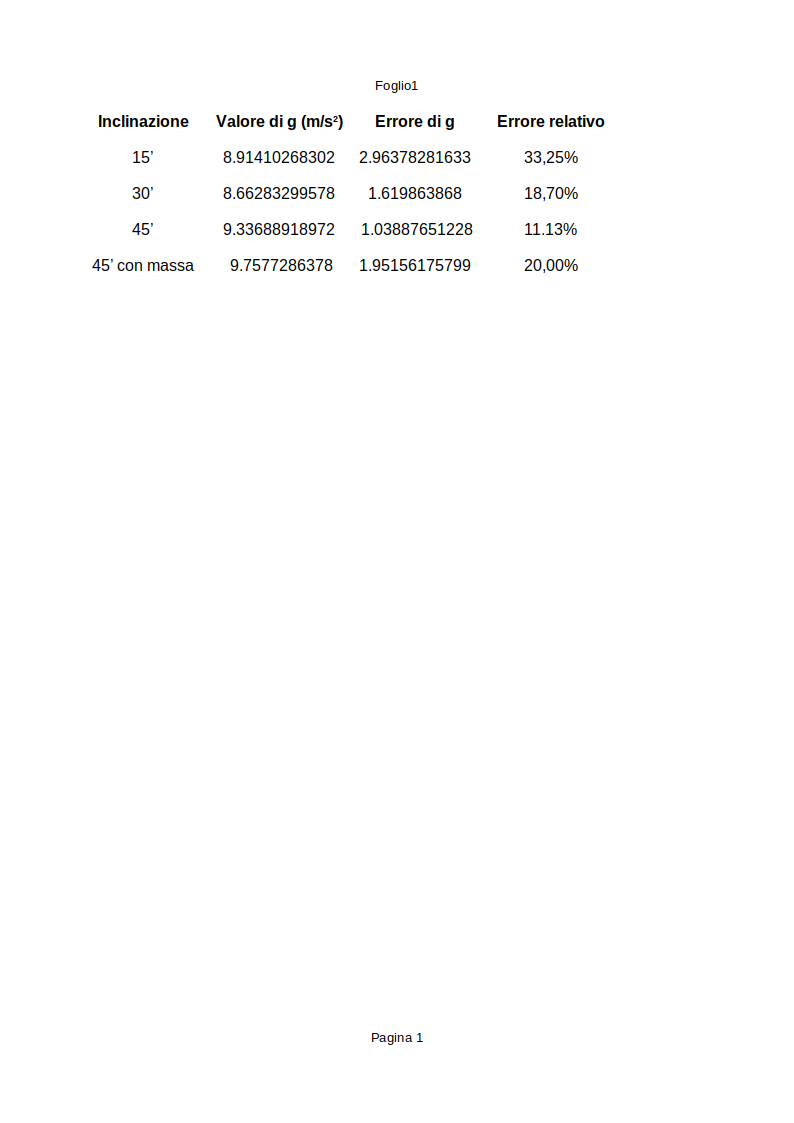
\includegraphics[scale=0.8]{valori di g.png} }
\end{figure}

\vspace{1cm}

\begin{figure}[h!]
\subfloat[Figura 2][valori di $g$ sistema asta-palo]{\includegraphics[scale=0.8]{valori di g brutto.png} }
\end{figure}



\vspace{1cm}
\begin{flushleft}
È stato così dimostrato che su un piano inclinato si presenta un moto rettilineo uniformemente accelerato e che le stime di accelerazioni effettuate sperimentalmente sono compatibili con il valore atteso a Padova, pari 9.806 \SI{\pm 1}{} $m/s$.

\end{flushleft}





\end{document}
